%  NOTE: Please make sure to completely fill out the \def parts in meta-data.tex!

\section*{Preface}

Foremost, I would like to express my gratitude towards all persons that helped me during the creation of this thesis. From helping me with finding the topic to helping me correct my mistakes while programming the algorithms used in this thesis. 
\\

I would like to especially thank my research supervisor \textbf{Dr. Dimitar Shterionov} (Assistant Professor and Researcher at Tilburg University) for the guidance given by helping me both with the research for this topic and correcting my many mistakes while coding. 

I am grateful to my fellow Thesis colleagues \textbf{Stan van der Vossen} (CSAI-Student), \textbf{Jakob E. Hauser} (CSAI-Student), \textbf{Stefano Scola} (CSAI-Student), and \textbf{Codrin Mironiuc} (CSAI-Student) for the advice, translating sporadic German to English, and guidance given towards solving the problems I faced during the creation of this Thesis.

Lastly, even though they are unaware of me writing this Thesis, I would like to express my gratitude towards all the researchers that aided in the creation of the DGS-Korpus and especially for making it available to the online public. \\ \\
\hfill
Gijs Thissen \\
Tilburg, May 2021

\newpage \thispagestyle{empty} \strut
\newpage \pagenumbering{arabic}

\title{\thesistitle{}}
\author{\yourname}

\maketitle % Yes, again

\begin{abstract}

Sign languages are languages that have unique grammar, words, and manners of speaking. Therefore they may be completely distinct from the regional equivalent spoken language. Most of the time these live in parallel worlds, with the deaf on one side and the hearing on another. When these worlds clash, confusion arises because of the dissimilarity between the two since they might not stem from the same language family. In recent years the field of neural machine translation has grown exponentially, with the invention of the transformer architecture increasing accuracy in machine translation software. German Sign Language (DGS) and German are two distinct languages and are therefore subject to translation possibilities. The recent approaches mainly focus on (German) text to (DGS) glosses. However,  there has been a lack of a glosses-to-text translation system. The focus of this paper is to find the best approach by adding temporal, vocal, or combined data to the glosses of the DGS Public Korpus. The results show that adding these extra tokens to the data results in a less accurate translation across all models. The neural machine translation system with an input of nothing but glosses [BLEU 3.69, TER 0.960] outperforms the more complex models [average BLEU 2.19, average TER 0.981]. It is concluded that adding temporal, vocal or both in the data without the use of standardization of the tokens aids in the emergence of more rare and unique words resulting in the decrease in accuracy of the model.

\end{abstract}

\section{Introduction}

Contrary to popular belief, sign language and spoken language are not the same. In fact, sign language has its own words and grammar (\citealp{camgoz2018neural}; \citealp{stokoe2005sign}) that are completely separate from its regional spoken counterpart. The earliest attested use of sign language can be found in Plato's Cratylus \cite{sedley2003plato}.  The hearing impaired, users of sign language, use signs as their day to day communication \cite{perniss2007}. This is done by the use of spatial-temporal gestures to communicate pieces of information.  However, communication between the signers and non-signers can prove to be difficult \cite{meadow1981interactions} when both of them do not know the other's language. 

\subsection{Spoken Language of the Deaf and Hard of Hearing}

When a deaf person signs, spoken words can be heard. In the field of sign language research, these spoken language utterances performed by deaf individuals are referred to as mouthings (\citealp{konradoffentliches}; \citealp{braem2001functions}). The concept of mouthings is quite common among non-deaf individuals. It is often referred to as intra-sentential code-mixing \cite{paradis2000early} and is fairly prominent among bilingual non-deaf children. However, bilingualism does not limit itself to solely hearing individuals. Many deaf persons are, in fact, bilingual. Only 8\% of deaf children are born to two deaf parents. Consequently, these children tend to "speak" both sign language and spoken language \cite{perniss2007}. Research suggests that in adults, this code-mixing has become a structural part of their linguistic abilities and plays an important role in the meaning of a sign. (\citealp{pfaff1979constraints};  \citealp{konradoffentliches}). It is, however, not consistent among sign languages. Signers of American Sign Language tend to use less mouthing when compared to signers of German Sign Language.

\subsection{Sign Translation}

When faced with situations where communication is key, written text is a solution to circumvent ambiguity. In the case of sign language, linguists have developed conventions for translating sign language into text (\citealp{konradoffentliches}; \citealp{aouiti2015arab}; \citealp{porta2014rule}). This is done by denoting a single gesture as a word. Around this word, several glosses are positioned.  Glosses are brief annotations used by linguists to denote an explanation of a word. For example, I LIKE [negative] COWS would translate to I don't like cows. Translating glosses to normal text is a tedious job that is exclusively done by specialised linguists. Preferably this task would be able to be automated. However, for this goal to be achieved, there is a need for a corpus to be machine-readable. Machine readability is achieved by making use of consistent sign annotations and tags \cite{johnston2008corpus}. 

To solve this problem, end-to-end machine translation models have been developed to recognize gestures and translate gestures directly to text \cite{de2020sign}. Sign recognition systems work by isolating different signs from each other, which has proven to be difficult due to the existence of a transitional period between signs \cite{konradoffentliches}  (See Section 3.4 about Segmentation for more details). While this approach has shown promising results it ignores the underlying linguistical aspects of sign language (\citealp{camgoz2018neural}; \citealp{perniss2007}). This paper will investigate whether or not adding temporal data improves machine translation systems for language glosses to text.

\subsection{Research Question}

\textbf{To what extent does temporal data aid in the performance of a machine translation system for sign language glosses to text?}
\\
The research question is broken down into the following sub-questions:
\begin{itemize}
    \item \textbf{How to introduce temporal data to the Machine Translation system?} \\
    The baseline system does not have temporal data added to it. This sub-question is related to how to add temporal data to the machine translation system.
    \item \textbf{To what extent does temporal data aid a Machine Translation system when compared to a baseline system?} \\
    The chosen dataset \cite{dgscorpus_3} contains both the glosses (i.e.: TO-HAVE-BSL1, I1\textasciicircum, BUTTER1A) and the timestamps next to them to indicate when and how long these signs have taken place. This sub-question is related to combining this temporal data with the baseline system. Both the baseline and the temporal experiments are described in the methods section.
    \\
    \item \textbf{To what extent does vocal data aid a Machine Translation system when compared to a baseline system?} \\
    The dataset contains both glosses on sign language and data on what the subject said during the interview (vocal). This sub-question is related to:
    \begin{enumerate}
        \item Combining the additional vocal data with the baseline system.
        \item Combining the additional vocal data with the temporal data and the baseline system.
        \item Measuring to what extent does adding extra tokens have an effect on the performance of the Machine Translation system.
    \end{enumerate}.
\end{itemize}

\subsection{Findings}

The results of the conducted research show that combining words and temporal features does not increase the accuracy of the model. Instead, combining these features decreases the BLEU score of the translated text by as much as 22\%. Even though prior research showed that mouthings are intrinsically part of a signer's linguistical ability (\citealp{pfaff1979constraints};  \citealp{konradoffentliches}) the results show a 45\% decrease in BLEU score when paired with words and fed into an NMT system. Combining all the data results in a BLEU score loss of 50\% on the translated text.

\section{Related Work}

Research on parallel translation of spoken language is widely attested. Sign language translation, however, is a relatively small field with little appropriate datasets or methods (\citealp{camgoz2021content4all}; \citealp{bragg2019sign}).

\subsection{Hidden Markov Models}
In the late 1990s, the field of Sign Language translation wasn't much of a separate field, the research that did exist was mainly focused on recognizing sign language. The focus of Sign Language Recognition mainly relied on HMMs (\citealp{hiddenmarkov1l}; \citealp{hiddenmarkov2}; \citealp{hiddenmarkov3}; \citealp{holden2005australian}). A gesture would be decomposed into a sequence of postures. These postures would then be recognised by the HMM as a gesture. For the system to be able to track a gesture the user would be wearing an annotation glove. For example, coloured rings would be worn around each finger. This approach changed in 1996 by using the colour of the participants' skin to segment from the background by calibrating the system on the participants noses \cite{starner1998real}. This proved to be problematic, however, since the hands move at a different pace compared to the nose the system would occasionally filter out the nose \cite{starner1998real}. In 2005, an end-to-end pipeline, called the Sign2 Conversion System \cite{glenn2005image}, was created. However, it could only be used for ASL finger-spelling excluding any non-alphabetical ASL signs and therefore limiting the system greatly by excluding essential linguistical aspects of the American Sign Language.

\subsection{Deep Learning}

Using neural networks in sign recognition was among the first methods proposed at the onset of the field (\citealp{murakami1991gesture}; \citealp{fels1993glove}), however, the approach was overshadowed due to the success of HMM's in the 1990s \cite{cooper2011sign}. The use of neural networks became more prominent in the late 2000s \cite{parton2006sign}. During this time several new international projects were set up to create sign language recognition systems for local sign languages (\citealp{ethopia}; \citealp{malaysia}; \citealp{persia}; \citealp{brazil}; \citealp{arabia}).  

Within recent times Deep Learning \cite{lecun2015deep} has gained popularity giving rise to new models. This enables the use of 3-dimensional convolutional neural networks. While previous recognition systems employed sign language recognition on 2-dimensional images, due to having no temporal dimension in their kernel this would result in a 2-dimensional output \cite{tran2015learning}. The main difference between the old systems and the new is the 3-dimensional convolutional neural network (CNN) that can extract discriminative spatial-temporal features \cite{huang2015sign}.

\subsection{Continuous Sign Language Recognition}

In mid 2010s the field has morphed into continuous sign language recognition (CSLR) \cite{koller2015continuous}. Where the older SLR systems were limited to the use of isolated gestures \cite{cooper2011sign}, through the use of (Long Short Term Memory) LSTM models \cite{hochreiter1997long} the field was able to create a CSLR system that recognizes gestures as a sequence of interconnected sub-units \cite{mittal2019modified}. This proved to be especially difficult since there are no clear boundaries between signs hands move from because signs do not simply stop but rather move in transitional movements (See Section 3.4 for details about Segmentation). An architecture that improves on this, even more, is the Transformer architecture \cite{vaswani2017attention} improving the WMT 2014 English-to-German translation task by 2 BLEU score (see Section 4.5 for details about BLEU) compared to older architectures. Consequently this architecture was applied to the field of SLR where Transformers have been proven to outperform LSTMs in SLR experiments (\citealp{de2020sign}; \citealp{camgoz2020sign}).

\subsection{Sign Language Translation}

The field of sign language recognition has continuously posed the problem of translating sign language as a purely symbolic one \cite{camgoz2018neural}. However, sign language is its own language with its own distinctive grammar (\citealp{perniss2007}; \citealp{camgoz2018neural}; \citealp{camgoz2020sign}), consequently by ignoring the grammar and linguistic properties of a sign language important information is lost. The current state-of-the-art solves this issue by using sequence-to-sequence based deep learning models. The SLR translation as performed by \citealp{koller2015continuous} is still performed, however, it is enhanced by embedding the glosses into the system \cite{camgoz2018neural}. Due to the lack of prior research into the topic of Sign Language Translation, especially regarding Neural Machine Translation, many tokenization methods have yet to be explored. In the NMT system, the temporal features are added, however, contrary to the signs and their respective glosses, no temporal data is embedded. Research has also shown that the mouthing a deaf person performs is of importance for the meaning of the sign that is being performed at the same time \cite{konradoffentliches}.
\\
\\
This thesis focuses on to what extent the addition of temporal or vocal tokens, aids in the performance of a gloss to text NMT system. The system will use the Transformer architecture in combination with source word features \cite{garcia2016factored} that correspond to either the temporal, vocal or combined glosses. The public DGS corpus \cite{dgscorpus_3} will be used due to the presence of both vocal and temporal tiers in the corpus. It is hypothesised that adding temporal, vocal, or either will progressively strengthen the NMT-system's accuracy while reducing the errors it makes in the translation.


\section{Data}

In the following section the source and distribution of the data for the NMT system will be discussed as well as the method in which the dataset was collected \cite{age_data_hamburg}. Furthermore, the conventions by which the corpus was created is presented and explained in detail.

\subsection{Source}

The data consists of $405$ EAF-files (ELAN Annotation Files) gathered by the Institute for German Sign Language and Communication of the Deaf at Hamburg University \cite{prillwitz2008dgs}. These files consist of a total of $50$ hours of annotated recordings spanning a wide range of narrations regarding the cultural aspects of the deaf community. The interviews were conducted using a peer-to-peer procedure, where participant change roles according to the conversation \cite{prillwitz2008dgs}. During a discussion $2$ German Sign Language or Deutsche Gebärdensprache (DGS) signers conversed. Each conversation consisted of a standardized interview covering linguistical and social data \cite{deaf_areas}. Following this conversation, a spontaneous conversation on a given topic was held while the participants were encouraged to use as much basic vocabulary as possible \cite{deaf_areas}. In the EAF-files the signers are annotated as either Speaker A or Speaker B. The data was collected between January $2010$ and December $2011$  by videotaping $330$ participants from all $16$ Federated States (Bundesländer). The recordings were conducted using a mobile field lab in; areas with a relatively high deaf population density (deaf schools, deaf centres, and deaf institutes) \cite{age_data_hamburg} \cite{deaf_areas}, the catchment areas of the former Schools for the Deaf (\citealp{age_data_hamburg}; \citealp{prillwitz2008dgs}), areas which were easy to reach from surrounding rural communities (\citealp{age_data_hamburg}; \citealp{deaf_areas}), and finally areas that were suspected of having a distinct dialect. (\citealp{age_data_hamburg}; \citealp{prillwitz2008dgs})


 The data was collected by representatives of the local deaf community to take into account the regional varieties of DGS \cite{deaf_areas}. As can be seen in \autoref{fig:bundeslander} the data was sampled from participants across different age groups \cite{age_data_hamburg}. 


% Age category figure
\pgfplotstableread[row sep=\\,col sep=&]{
    interval & carT & carD \\
    18--30     & 12.1  & 12.4  \\
    31--45     & 13.6 & 13.9  \\
    46--60   & 12.7 & 12.4 \\
    61+   & 11.5 & 11.2 \\
    }\mydata

\begin{figure}[h]
\caption{Showing the percentage of participants per age, divided into both the Male (shown in Purple) and Female (shown in Red) gender,  that participated in the creation of the DGS corpus (both annotated and non-annotated).  \cite{age_data_hamburg}}
\begin{tikzpicture}
    \begin{axis}[
            ybar,
            title={Age distribution in The DGS-Korpus project sample (Percentage Vs. Age Categories)},
            bar width=.6cm,
            width=.8\textwidth,
            height=.5\textwidth,
            legend style={at={(0.5,1)},
                anchor=north,legend columns=-1},
            symbolic x coords={18--30,31--45,46--60,61+},
            xtick=data,
            nodes near coords,
            nodes near coords align={vertical},
            ymin=0,ymax=25,
            xlabel={\/Age categories},
            ylabel={\/Percentage of participants (\%)},
        ]
        \addplot table[x=interval,y=carT]{\mydata};
        \addplot table[x=interval,y=carD]{\mydata};
        \legend{Male, Female}
    \end{axis}
    
\end{tikzpicture}

\label{fig:bundeslander}
\end{figure}

\subsection{ELAN}
The conversation conducted between the representatives of the deaf community has been annotated and stored in EAF-files. These EAF-files can be shown and edited using the ELAN software \cite{crasborn2008enhanced}. ELAN is a multimedia annotation software developed by \citep{elan_software} to assist in Linguistical studies, language conservation, and sign language research \cite{brugman2004annotating}. The software can be used to add annotations to video and/or audio recordings. An annotation can be a sentence, word, or in the case of sign language, a gloss. Using ELAN multiple annotations can be created that are sorted into tiers \cite{crasborn2008enhanced}.  

% EAF-example
\begin{figure}[h]
\caption{Showing the structure of one of the EAF (English Annotated File)-files \cite{elan_example} inside the program ELAN. ELAN is a multimedia annotation tool used for multi-modality research \cite{sloetjes2017elan}. }
 \centering 
 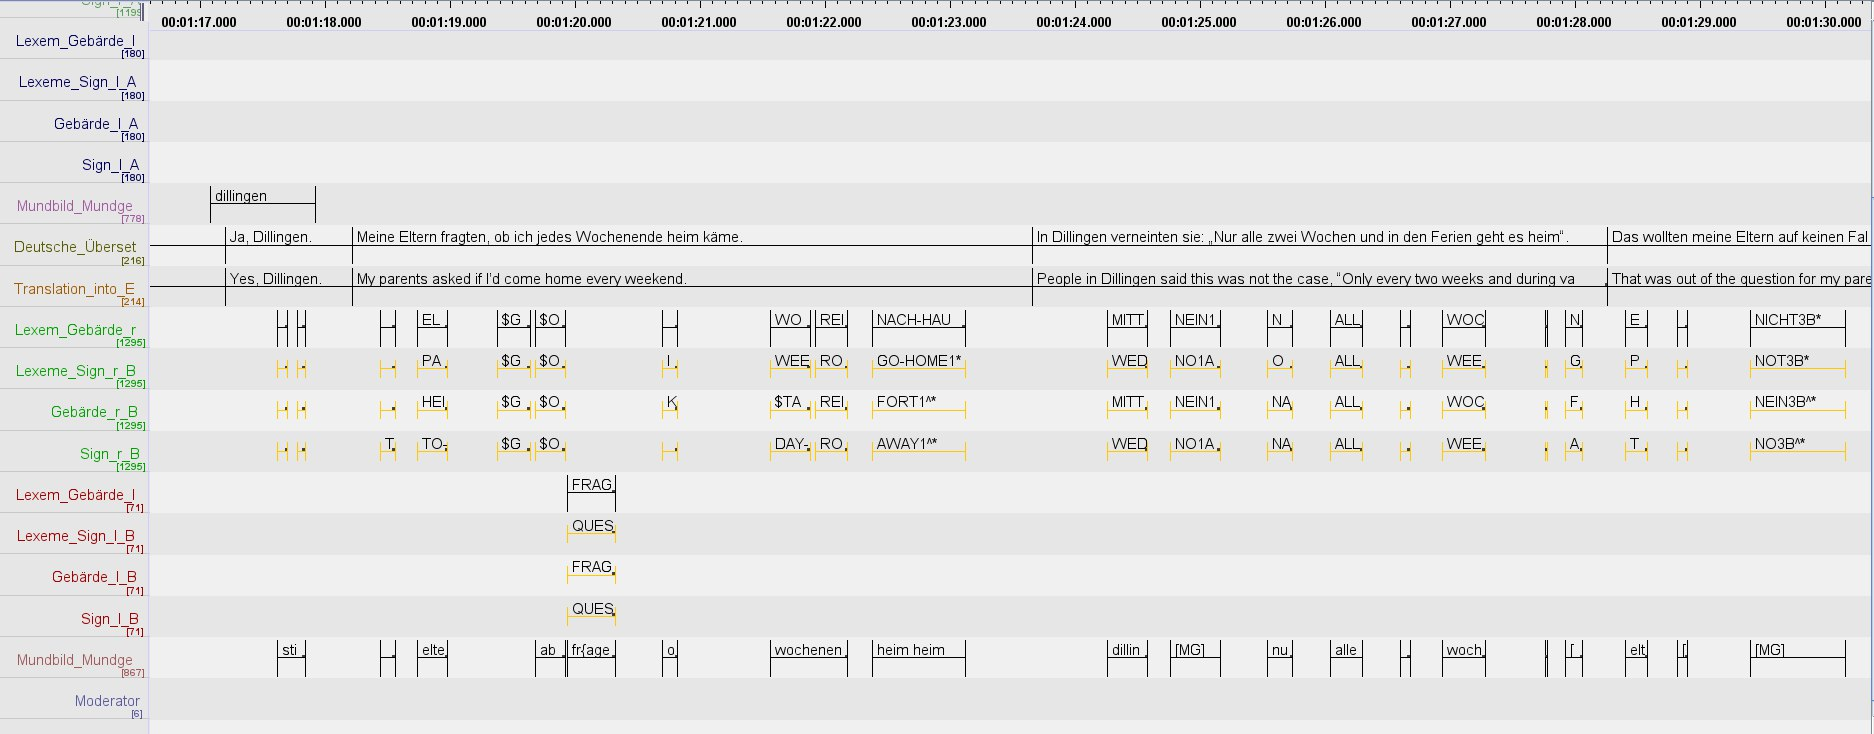
\includegraphics[width=14cm]{Bachelor CSAI thesis template/images/ELAN_example.jpg}
 
 \label{fig:elan_example}
\end{figure}

\subsection{Initial Translation}

The annotations are divided into tiers are presented across a timeline. As can be seen in (\autoref{fig:elan_example}) these files are divided into $11$ different tiers, presented in both English and German due to accessibility \cite{konradoffentliches}. Take "Lexem\_Gebärde\_r\_A" for example, this tier is translated into English as "Lexeme\_Sign\_r\_A". The tiers present in the EAF-files, translated into English, are: "Time", "Sign\_l\_B", "Sign\_r\_B", "Lexeme\_Sign\_l\_B", "Lexeme\_Sign\_r\_B", 
"Translation\_into\_English\_B", "Sign\_l\_A", "Sign\_r\_A", "Lexeme\_Sign\_l\_A", "Lexeme\_Sign\_r\_A", and "Translation\_into\_English\_A" \cite{sloetjes2017elan}. The goal of this research is to investigate to what extent temporal data aids in the performance of a machine translation system for sign language glosses to text. For this purpose, both the German Sign Language and the German Language were chosen respectively. Since the target language is German, since the corpus originated at the university of Hamburg \cite{age_data_hamburg}, it was decided to use the original glosses and translations that were available in the corpus. 

The initial translation of the glosses in the data set (i.e.: Sign\_l\_A to Translation\_into\_English) was conducted by contracted sign language translators and interpreters \cite{konradoffentliches}. These researchers translated the data set word-for-word. Consequently, university students created coherent meaningful sentence like structures. Lastly, these sentences were fed back into the system until the proper meaning was determined by the DGS experts (\autoref{fig:uselesspipeline}) \cite{konradoffentliches}.

\begin{figure}[h]
\caption{Showing the translation pipeline of the initial translation phase as conducted by the Institute for German Sign Language and Communication of the Deaf at Hamburg University. \cite{konradoffentliches} }
 \centering 
 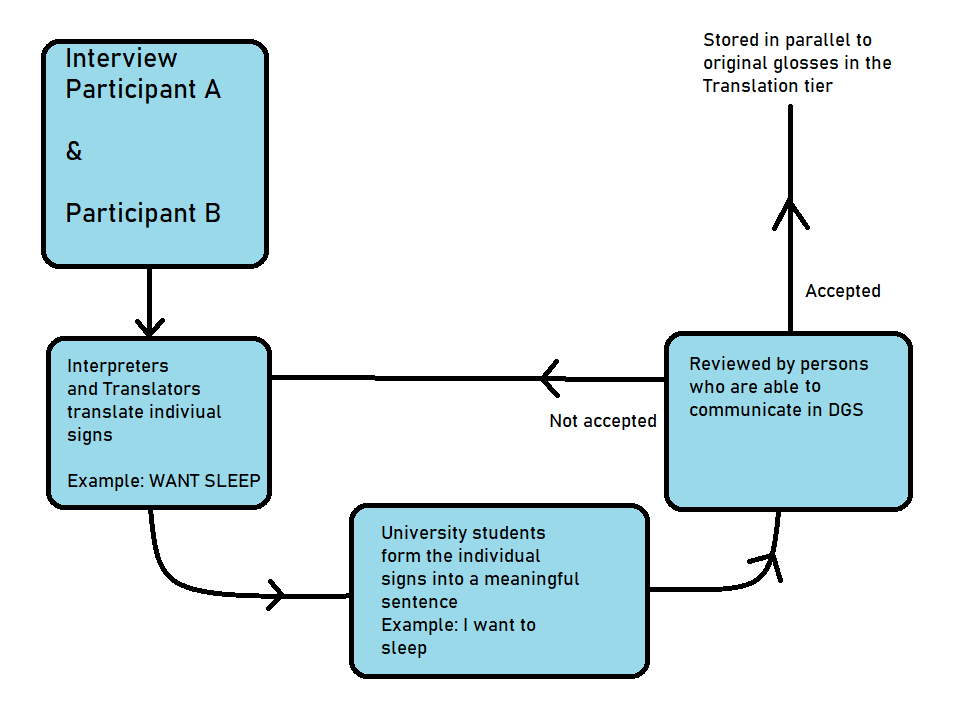
\includegraphics[width=14cm]{Bachelor CSAI thesis template/images/translation_pipeline.png}
 
 \label{fig:uselesspipeline}
\end{figure}

\subsection{Segmentation}

As with spoken languages, sign languages tend not to have a naturally occurring white space character (\citealp{hankesegmentation}; \citealp{konradoffentliches}). Thus it is difficult to determine where a sign begins and where a sign ends. In this situation, the segmentator has two options: either add a gap or none at all. Unlike spoken languages, when a participant is signing two words, take TREE (rest your right forearm upon your left palm and twist) \cite{perniss2007space} and COW (make two horns using your thumb and little finger on top of your head), for example. There is a transitional period where the participant moves his or her arm from one sign to the next. When adding a gap between the signs, the segmentator determines that the transitional movements are not part of the token's form \cite{konradoffentliches}. Taking this into account researchers at the University of Hamburg have decided that for the creation of the DGS corpus gaps will be added. The direct result of this decision is located in the EAF files, where there is temporal data assigned to the white spaces.

\subsection{Lemmatisation and Gloss conventions}

When creating a corpus there is an intrinsic need to have conventions in place to make sure a uniform dataset is created \cite{konradoffentliches}. Therefore it is necessary to employ linguistics to standardise glosses using gloss conventions \cite{kristoffersen2016designing}:

\begin{itemize}
    \item In the field of Linguistics or more specifically in the field of lexicography, a lexical item forms the basic element of the lexicon of a language. Lexical signs are treated as items, that is as units of their respective sign language that would be found in the dictionary \cite{konradoffentliches}. When a deaf person signs SQUARE1\textasciicircum  it may mean different things such as a map, a recipe, or a page. In DGS \cite{perniss2007space} and several other European Sign Languages signs are iconically motivated (\citealp{pietrandrea2002iconicity}; \citealp{oomen2017iconicity}), meaning that there is a similarity between the form of the sign and the meaning of the sign. In the DGS corpus, type glosses are given an indication of iconic value by using a circumflex at the end: "SQUARE1\textasciicircum ". Examples of child types to the SQUARE1\textasciicircum parent type are: FORM1, MIRROR2, and PAPER4, these and all other non-circumflex glosses are subtypes. The numbers denote different lexical variants.
    \item Fully iconically motivated signs, also known as poly-morphemic signs, are denoted as productive signs in contrast to lexical signs that denote a object in nature instead of meaning. Productive signs, therefore, have a \$PROD token \cite{konradoffentliches}
    \item Due to the anonymisation laws present in Germany, where this corpus was created, all names are replaced by "\$NAME". Except when it concerns a famous person the \$NAME gloss is followed by the person's name. \cite{konradoffentliches}
    \item Foreign language elements are represented using the INTS token, for example, when signing the English word Germany instead of "Deutschland" it has been written as GERMANY-INST1. (\citealp{kellett2008english}; \citealp{konradoffentliches})
    \item In German Sign Language it is conventional to use a one-handed manual alphabet, for example when spelling out someone's name. For these situations, the \$ALPHA token is used. Numbers are presented similarly by using \$NUM. \cite{konradoffentliches}  
\end{itemize}

Taking into account these points a uniform corpus was created with annotated signs presented on a timeline. An example of an annotated DGS sentence can be seen in \autoref{fig:sentence_example}.

\begin{figure}[h]
\caption{Showing an example sentence of the annotated corpus in DGS glosses. The German translation of this gloss sentence is: "Und dann fällt es einem wieder auf, dass der andere noch Fehler macht" \cite{dgscorpus_3}. (English translation: And then one notices again, that the other (person) is still making mistakes). 1. A token denoting a gesture. 2. The sign annotated as NM has iconic meaning. 3. One of several lexical variants of the lexical unit FEHLER.}
 \centering 
 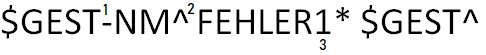
\includegraphics[\textwidth]{Bachelor CSAI thesis template/images/sentence_example.png}
 
 \label{fig:sentence_example}
\end{figure}

\section{Methods}

Since the data was created under specific gloss conventions \cite{konradoffentliches} it is difficult to build a MT system with. Furthermore, the data was split up into multiple separate files and it was therefore necessary for these files to be ordered and combined. This section will show the various techniques that were employed in this process.

\subsection{Experiments}

To answer the (sub-) research questions, experiments are needed. Described below are $4$ experiments that have been designed to test the hypotheses, they differ mainly in the data structure. A good overview of their differences can be found in (\autoref{fig:baseline_comparison}). 

\subsubsection{Baseline}

Other experiments will be compared to the baseline. This model lacks any externally added tokens. The data consists of a sequence of glosses as the source and their German translations as the target (Source: PRIVAT1A* FAMILIE1 Target: Privates oder Familie? \cite{dgscorpus_3}). The sign language glosses are without any transitional periods (See the Lemmatisation and Gloss conventions section in Data) and adhere to the standard gloss conventions.


\subsubsection{Temporal}

One of the sub-goals of this thesis is to, inspect or identify to what extent temporal data aids in the performance of machine translation systems for sign language glosses to text. This will be tested in the Temporal experiment. The data in the temporal experiment consists of the glosses formed into a sentence with tokens added to each word separated by the "|" character, e.g.: FAMILIE|120. The number behind the | character represents the total amount of milliseconds it took for a sign to be signed, in the given example this would mean that the sign for FAMILIE (English: Family) would have taken 120 ms to be made. As mentioned before these sentences are without the transitional periods from one sign to another (See Section 3.5). The "|" sign is a library standard sign to split Word features from the actual words \cite{klein-etal-2017-opennmt}. The temporal data files consist of glosses formed into a sentence with added temporal data and their German translation as the target (Source: PRIVAT1A*|340 FAMILIE1|460 Target: Privates oder Familie? \cite{dgscorpus_3})

\subsubsection{Vocal}

Another sub-goal of this thesis is to investigate to what extent adding extra embeddings aids in the performance of machine translation systems for sign language glosses to text. This will be tested in both the Vocal and the Combined experiment. The data in the vocal experiment consists of glosses formed into a sentence with tokens added to each word that represent the spoken words uttered by the participant while performing this sign. Research has shown that the mouthing a deaf-person performs is of importance for the meaning of the sign that is being performed at the same time \cite{konradoffentliches}. The spoken word and the gloss will be separated by the "|" character as per library standard \cite{klein-etal-2017-opennmt}. When using the OpenNMT library \cite{klein-etal-2017-opennmt} it is necessary that all source word features have the same amount of features. Thus when a sign does not have an accompanied mouthing a "nan" will be added instead of the spoken word. This is done to represent the empty space created by the empty row. The vocal data files consist of glosses formed into a sentence with added vocal data and their German translation as the target (Source: PRIVAT1A*|privat FAMILIE1|familie Target: Privates oder Familie?). It is important to note that all vocal word features are denoted solely using lowercase characters.

\subsubsection{Combined}

Research has shown that talking speed is affected by emotions \cite{kshirsagar2002multilayer}. The combination experiment is an experiment that combines the previously mentioned temporal and vocal features into one model.  The data will be separated by a "|" and be processed in a GLOSS|vocal|TIME format. The same conditions apply to the combined model as applied to the vocal and temporal model. The combined data files consist of glosses formed into a sentence with added vocal and temporal data and their German translation as the target (Source: PRIVAT1A*|privat|340 FAMILIE1|familie|460 Target: Privates oder Familie? \cite{dgscorpus_3}).

\begin{figure}[h]
\caption{Showing the source file textual comparison between the Baseline, Temporal, Vocal, and Combined experiments. In the temporal experiment, the concept of time is added (in ms). In the vocal experiment, the concept of spoken words is added (in lowercase letters). In the combined experiment these are combined into one.}
 \centering 
 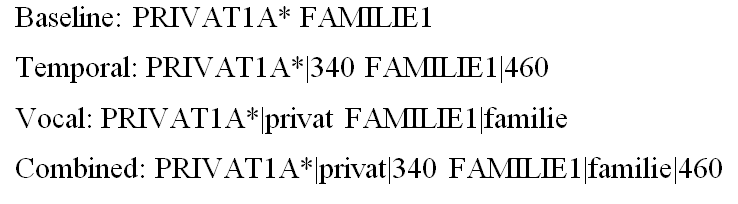
\includegraphics[width=14cm]{Bachelor CSAI thesis template/images/baseline_compared.PNG}
 
 \label{fig:baseline_comparison}
\end{figure}


\subsection{Pre-Processing}

\subsubsection{EAF to CSV}
Using the ELAN software $7$ of the $11$ tiers were selected and converted into a CSV file. This creates $2$ distinct CSV files that were consequently merged (\autoref{apx:first}). Due to having merged the files, there are no longer multiple persons in the data set, instead, the data set is transformed into a contextless database. Due to being able to access the timeline in ELAN \cite{elan_software}, it is possible to extract the temporal features of a given annotation. As mentioned before the annotators decided to add gaps between the signs (\citealp{hankesegmentation}; \citealp{konradoffentliches}), this has been carried over into the EAF-files, resulting in empty rows inside the CSV file. These need to be removed since the program automatically puts white spaces between words instead of pasting them into one giant string (\autoref{apx:first}). Failing to do so would result in temporal features being assigned to empty strings (A temporal-annotated sentence without removal of prior white spaces would result in \$GEST-NM\textasciicircum|430 |230 FEHLER1*|450 |400 \$GEST\textasciicircum|400).

\subsubsection{Data splitting}

As has been described $4$ experiments are to be performed: Sign, Temporal, Vocal, and Combined. For each of these experiments, two files are needed: a Source file (.src), and a Target file (.trg). These files are fully extracted from the data frame. By isolating the sentences in the data frame it is possible to create a separate sentence set for every sentence. This will result in $5$ files: normal.en, vocal.en, times.en, combined.en and sentences.nl. "sentences.nl" is the target file for all the experiments and is therefore uniform.

To tokenize and split the data the \texttt{train\_test\_dev.py} \cite{dimitarshterionovtrain} script was used to both tokenize and split the data into a training, a validation, and a testing file. Since the data set only has $60000$ sentences it was decided to split the data into only 500 sentences for validation and testing each while the remaining $59000$ sentences were used for the training file.

An unwanted side-effect of the \texttt{train\_test\_dev.py} \cite{dimitarshterionovtrain} script is that it adds white spaces between the individual sentences in both the (train, test, dev) source files as the target files. This results in the Machine Translation system "assigning" sentences to these white spaces when training, resulting in a normal German sentence within a normal German sentence. For this reason all files are passed through the \texttt{remove\_whitespace.py} script (\autoref{apx:fixing}) which will strip away all empty lines. 


\subsubsection{BPE}

Byte Pair Encoding (BPE) is a general-purpose data compression algorithm \cite{gage1994new} which has been employed for MT to reduce the OOV instances \cite{sennrich2015neural}. The way it works is by replacing the most frequent pair of bytes in a sequence with unused bytes, in the case of the OpenNMT Byte Pair Encoding \cite{klein-etal-2017-opennmt} scripts the unused bytes were denoted in the data files as "@@ ". The advantages of using the BPE algorithm are:

\begin{enumerate}
    \item \textbf{Memory}. In the case of German, many words start with the unit "auf", by encoding this unit by only using $1$ symbol, the system only encounters one symbol instead of $3$. \cite{gage1994new}
    \item \textbf{Out-of-vocabulary words (OOV)}. Taking into account the previous example, since the sub-unit "auf" has been replaced by $1$ symbol encountering it will be familiar. This is because BPE allows for the encoding of rare words and will not introduce any unrecognised tokens. When the system thenceforth encounters words containing the sub-unit it will be more familiar rather than it would be in the case without the sub-unit. (\citealp{gage1994new}; \citealp{sennrich2015neural})
\end{enumerate}

Before being passed to the pre-processing and training, the data, with the exception of the test.trg-file, since after translation the output file will be passed through an un-encryption algorithm resulting in normal text, were passed through a modified form of the BPE algorithm.  In normal circumstances when using BPE, it caused no problems, however, when applying BPE to data containing temporal word features it would split the word on the "|" character. The modified algorithm first double-checks whether or not there is a temporal feature added to the word and if there is will join the word and its respective temporal feature together (\autoref{apx:bpemod}). Applying \texttt{remove\_whitespace.py} on the data files significantly increases the BLEU-score for the Baseline model, while the old Baseline (pre-BPE, post-removal) had a BLEU score of 2.15, the new Baseline (post-BPE, post-removal) had a BLEU-score of 3.69. It was therefore decided to use the Byte Pair Encoding algorithm to compress the data files.  


\subsection{OpenNMT}
 
To train the data a Neural Machine Translation library is needed that supports source word features. With these criteria in mind $2$ libraries were eventually found: OpenNMT \cite{klein-etal-2017-opennmt} and MarianNMT \cite{mariannmt}. A main difference between the two remaining libraries is the way source word features can be used. Consider the following sentence: "PRIVAT1A*|340 FAMILIE1", as can be seen, the first word has word features attached, however, the second word does not. While this is not a problem in MarianNMT this would be a cause a problem in OpenNMT since it's source word features need to be consistent. Nonetheless, OpenNMT was chosen as the preferred library because of its compatibility with Microsoft Windows $10$. 

\subsection{Hyperparameters and Architecture}

Using OpenNMT \cite{klein-etal-2017-opennmt} a Transformer model was trained. The hyperparameters were picked to match the recommended standard transformer hyper-parameters \cite{standard_hyperparameters} as shown in (\autoref{tab:parameter}). These settings were chosen to create a model that is able to imitate the WMT2014 German-English \cite{WMT2014} results as achieved by the original paper on Transformers \cite{vaswani2017attention}. Overfitting on a small data set (the training data consists of $60000$ sentences) is a major challenge \cite{barone2017regularization}, therefore,  an early stopping criterion was introduced. If the perplexity and accuracy of the model do not improve during the last 5 validation performances the system will be stopped. Due to the limited capabilities of the system used, even with the use of the BPE algorithm, the batch size had to be decreased from a recommended 4096 to 1024.



\begin{table}[h]
\caption{Showing the hyperparameters used for training using the Transformer architecture.}
\centering
\begin{tabular}{|ll|ll|}
\hline
\multicolumn{1}{|l|}{Hyperparameter} & Setting     & \multicolumn{1}{l|}{Hyperparameter} & Setting              \\ \hline
Encoder type                    & Transformer & Batch size                     & 1024                 \\
Decoder type                    & Transformer & Batch type                     & tokens               \\
Transformer feed-forward        & 2048        & Normalization                  & tokens               \\
Layers                          & 6           & Warm-up steps                  & 8000                 \\
Heads                           & 8           & Training steps                 & 20000                \\
RNN size                        & 512         & Validation steps               & 1000                 \\
Word embedding size             & 512         & Label smoothing                & 0.1                  \\
Position encoding               & True        & World size                     & 1                    \\
Maximum generator batches       & 2           & GPU rank                       & 0                    \\
Dropout probability             & 0.1         & Early stopping                 & 5                    \\
Optimization method             & adam        & Early Stopping criteria        & perplexity, accuracy \\
Adam beta2 hyperparameter            & 0.998       & Max gradient norm              & 0                    \\
Decay Method                    & noam        & Parameters initialized at      & 0                    \\
Learning rate                   & 2           & Parameters\_init\_glorot       & True                 \\ \hline
\end{tabular}

\label{tab:parameter}
\end{table}

\section {Evaluation Metrics}
\subsection{BLEU}

BLEU is short for Bilingual Evaluation Understudy and is an evaluation metric for Neural Machine Translation as described in \cite{papineni2002bleu}. As the name suggests it is an evaluation metric for a parallel bilingual system with a reference (original target file) and a hypothesis (predicted target file). Previously used metrics were human-based and could take weeks or even months to be calculated \cite{papineni2002bleu}. The idea behind the metric was that the closer a machine translation was to a professional (linguistic) human translation, the better it was. Therefore one has to measure how close the prediction is to the reference translations.

\subsubsection{Weighted precision}
BLEU uses the weighted precision score (\autoref{fig:weighted_precision}). The difference between the modified version and the normal version is that the modified version takes into account the maximum reference count \cite{chan}. If the "normal" precision measure was used with multiple references, when comparing the sentence "dog dog dog dog dog dog dog" with "I want a dog" would be able to get a score of close to 1. This is especially true since MT systems tend to over-generate words that seem to fit in \cite{papineni2002bleu}.


\begin{figure}[h]
\caption{Showing the modified n-gram precision formula. The difference between the modified version and the normal version is that the modified version takes into account the maximum reference count, known as the clipped count. Candidates refers to the translated sentences \cite{chan} \cite{papineni2002bleu}. First compute the N-gram matches. Second add the clipped counts for all translated sentences. Third divide the sum by the total number of n-grams in the reference. \cite{chan}}
 \centering 
 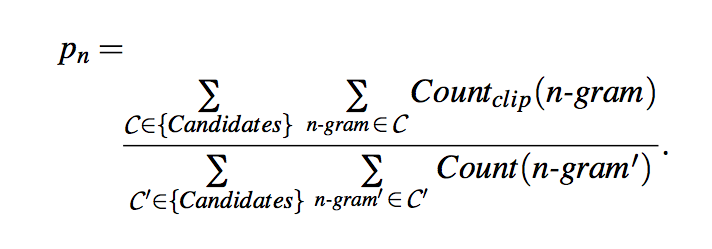
\includegraphics[width=10cm]{Bachelor CSAI thesis template/images/weighted_precision.png}
 \label{fig:weighted_precision}
\end{figure}

\subsubsection{Brevity penalty}
Traditionally the BLEU-score was used to calculate the score of a prediction over multiple references. Since these references may or may not have variable length this will negatively affect the recall score \cite{papineni2002bleu} (Section 2.2). The proposed solution is the brevity penalty or BP for short as can be seen in (\autoref{fig:full_bleu}). The Brevity penalty high scoring translations must match the references in word order and length. Sentences smaller than the reference sentences are therefore penalized since they are multiplied by a factor < $1$. 


\begin{figure}[h]
 \caption{Showing the complete formula for calculating BLEU \cite{papineni2002bleu}. In the BP formula, c denotes the total length of the translation corpus, r is the sum of the best match lengths of the translation sentence in the test corpus \cite{papineni2002bleu}. If the BP value is 1 this means that the translation length and the reference length are equal if this is not the case the second formula will be used. The eventual BLEU-score is the average of the weighted precision scores times the brevity penalty and therefore penalizes shorter sentences. }
 \centering 
 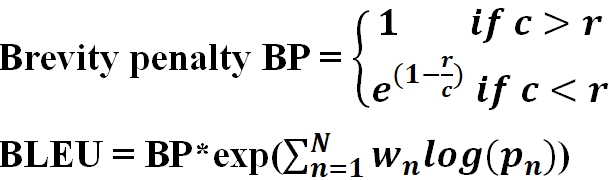
\includegraphics[width=8cm]{Bachelor CSAI thesis template/images/bleu_formula.PNG}
 \label{fig:full_bleu}
\end{figure}

\subsubsection{BLEU-score}

The BLEU score ranges from 0 to 1, with 0 being not related to the reference sentence and 1 being identical. As a convention in the field of Neural Machine Translation, the BLEU-score is either multiplied by 10 or 100, for the purposes of this paper the BLEU-score will be multiplied by 100. In this paper, BLEU will be used on only $1$ reference since there is only one available per gloss sentence.

\subsection{TER}

Translation Edit Rate (TER) measures the amount of editing that needs to be done to create an output that exactly matches a reference translation \cite{TERsnover2006}. There can be multiple TER-scores since they may match one of many references, however, since in this paper only one reference will be used this will not be considered a problem. The higher the TER-score the worse the translation, since the more edits are performed on the total number of edits. The formula to calculate the TER-score is shown in (\autoref{fig:full_ter}). The number of edits is calculated in two different phases \cite{shapira2002edit}:
\begin{enumerate}
    \item A greedy search algorithm is used to find the words that need to be shifted from one place to another.
    \item An optimal calculation is made to calculate the smallest amount of remaining edits (insertion, deletion, and substitution) necessary to match the reference.
\end{enumerate}



\begin{figure}[h]
 \caption{Showing the formula for calculating the TER score \cite{TERsnover2006}. The TER-score is calculated by dividing the number of edits by the average number of words in the reference translation. Possible edits are insertion, deletion, substitution, and switching words around. All these edits have an equal cost.}
 \centering 
 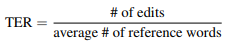
\includegraphics[width=7cm]{Bachelor CSAI thesis template/images/ter_formula.PNG}
 \label{fig:full_ter}
\end{figure}


\break

\section{Results}

\begin{table}[h]
    \caption{Best performing models with the accompanying BLEU- and TER-scores. Highlighted in bold are the best results. As can be seen in the table the baseline outperforms all other models.}
    \label{tab:results}
    \begin{tabular}{llrr}
        \toprule
                                                                  
        Word-Form                   &  Models                           &  BLEU                & TER    \\ 
        \midrule
        \multirow{3}{*}{Original}  &  Baseline                              &   \textbf{3.69}      &  \textbf{0.960} \\
                              & Temporal                                &   2.85               &  0.971 \\
                              & Vocal                                   &   2.03               &  1.000 \\
                              & Combined (Temporal + Vocal)             &   1.69               &  0.973 \\
    
        
    \end{tabular}
    
\end{table}


At the beginning of this paper it was hypothesised that with the insertion of temporal data into the baseline data, there would be an improvement of the translation quality. Additionally, it was hypothesised in a sub-hypothesis that the addition of a vocal token would increase the BLEU-score of the model (see Section 4.1.3 on the scientific background). For these reasons $4$ experiments were set up, the baseline, temporal (baseline + time), vocal (baseline + vocal), and combined (baseline + vocal + time). These experiments were performed, on each of them, their respective BLEU and TER score were calculated these results are presented in (\autoref{tab:results}). Histogram plots are shown in Figure 9 and 10 to compare the scores to each other and see any possible trends between them.

\subsection{Baseline fine-tuning}

The baseline experiment consisted of $4$ sub-experiments, the results are shown in (\autoref{fig:hyperparameter}). The first experiment that was run, ran on basic hyperparameters, such as a learning rate of 0.01, however, this architecture was abandoned in favour of mimicking the original transformer architecture. The results improved by 17.6\% (1.12 -> 1.36). The fine-tuning of the third experiment had to do with the pre-processing. In both the first and second experiment an oversight was made regarding empty lines in the data files, these would result in sentences being learned for empty source lines. Applying \texttt{remove\_whitespace.py} on the data files significantly increases the BLEU-score for the Baseline model, while the old Baseline (pre-BPE, pre-removal) had a BLEU score of 1.36 the new Baseline (pre-BPE, post-removal) had a BLEU score of 2.15. The algorithm improved the results by 36.7\% (1.36 -> 2.15), it was therefore decided to use the \texttt{remove\_whitespace.py} on all data files. The fourth and final experiment was tuned by applying the BPE algorithm \cite{gage1994new} (see section 4.2.3). The results improved by a total of 41.7\% (2.15 -> 3.69). The translated text of the final baseline translation model had a BLEU-score of 3.69 and a TER score of 0.960, an example is shown in (\autoref{tab:baseline_translation}). The former is an improvement of 69.6\% compared to the non-tuned baseline while showing a general trend of improvement across the sub-experiments. When the BLEU-score is 3.69 and the TER score 0.960 are compared to contemporary research they are below average.  However, of the $4$ conducted experiments the baseline model had the best performance.

\begin{table}[h]
\centering
\caption{Showing the translation results of the baseline model, the original input is the input of the glosses in accordance to the gloss conventions. While the test reference sentence is more strict and solely presents a sentence using und and oder. The predicted sentence is more in the context of the conversation about deafness. }

\begin{tabular}{ll}
\textbf{Original Gloss Input}     & MAMA1A* PAPA8* \$GEST\textasciicircum{} PAPA1B* OMA1C* \\
\textbf{Model Predicted Sentence} & Meine Mutter und mein Bruder, der ja auch hörend war.                                                                                     \\
\textbf{Test Reference Sentence}  & Ja, MAMA und PAPA, oder so PAPA, PAPA, OPA, OMA.                                                                                         
\end{tabular}
\bottomrule
\label{tab:baseline_translation}
\end{table}

\pgfplotstableread[row sep=\\,col sep=&]{
    Model &      carT         \\
    1st     & 1.12  \\
    2nd     & 1.36  \\
    3rd   & 2.15      \\
    4th   & 3.69    \\
    }\mydata

\begin{figure}[h!]
\caption{Showing the BLEU-scores from the $4$ performed sub-experiments. The description of the experiments can be found in section 5.1. Overall there is a trend of improvement along with the fine-tuning of the model.  On the X-axis the different models are presented. On the Y-axis the score is shown, the calculation and description of the BLEU score is described in Section 4.5)}
\begin{tikzpicture}
    \begin{axis}[
            ybar,
            title={Improvements of the baseline (BLEU-Score vs. Model)},
            bar width=.6cm,
            width=.8\textwidth,
            height=.5\textwidth,
            legend style={at={(0.5,1)},
                anchor=north,legend columns=-1},
            symbolic x coords={1st, 2nd, 3rd, 4th},
            xtick=data,
            nodes near coords,
            nodes near coords align={vertical},
            ymin=0,ymax=4,
            xlabel={\/Models},
            ylabel={\/Score},
        ]
        \addplot table[x=Model,y=carT]{\mydata};
        \legend{BLEU-score}
    \end{axis}
    
\end{tikzpicture}

\label{fig:hyperparameter}
\end{figure}

\subsection{Experiments}

The second experiment was performed to answer the question of whether or not adding temporal data into the source files would aid in the performance of the model. The translations generated by the temporal model received a BLEU-score of 2.85 and a TER of 0.97. When compared to the baseline system this a decrease of 22.8\% in BLEU-score and a similar TER score, an example of a generated translation can be seen in (\autoref{tab:temporal_translation}). 

\begin{table}[h]
\centering
\caption{Showing the translation results of the baseline model, the original input is the input of the glosses in accordance with the gloss conventions with embedded temporal features denoted by |NUMBER. The model seems to break down while translating, repeating the same word "Mama" over and over again.}

\begin{tabular}{ll}
\textbf{Original Gloss Input}     &MAMA1A*|120 PAPA8*|340 \$GEST\textasciicircum{}|60 PAPA1B*|260 OMA1C*|120  \\
\textbf{Model Predicted Sentence} & Das ist meine Mama und meine Mama und meine Mama meine Oma  \\     
\textbf{Test Reference Sentence}  & Ja, MAMA und PAPA, oder so PAPA, PAPA, OPA, OMA.              \\                       \bottomrule                                                    
\end{tabular}

\label{tab:temporal_translation}
\end{table}

The third experiment was performed to answer the question of whether vocal data would aid in the performance of the baseline model. The results show a BLEU-score of 2.03 which is a decrease of 45.0\% compared to the baseline. The calculated Translation Error Rate on the model is 1, the maximum rate since TER-scores are between 0 and 1, suggesting that a high number of edits was necessary to reach the reference. A practical example of this can be seen in (\autoref{tab:vocal_translation}). Research, however, suggests vocal utterances of deaf individuals are a strong indication of meaning \cite{konradoffentliches}.

% ----------------------------
\begin{table}[h]
\centering
\caption{Showing the translation results of the vocal model, the original input is the input of the glosses in accordance with the gloss conventions with embedded vocal features denoted by |mouthing. The sentences of the model seem to be quite a bit more basic as compared to the baseline and temporal experiments.}

\begin{tabular}{ll}

\textbf{Original Gloss Input}     & GUT1*|nan TOLL1A|toll GLÜCK1*|glück GUT1*|nan \\
\textbf{Model Predicted Sentence} & Das war sehr gut.                                                                                     \\
\textbf{Test Reference Sentence}  & Gut, das ist toll. Du hattest Glück.        \\                                      
\bottomrule
\end{tabular}

\label{tab:vocal_translation}
\end{table}

% --------------------------

The final experiment was performed to answer the question of whether or not combining the third and fourth experiment would aid in the performance of a gloss to text machine translation system. Results show a BLEU-score of 1.69, which is a decrease of 54.2\% compared to the baseline. The calculated TER on the model is 0.97, while a small increase compared to the baseline. Surprisingly, however, while being worse compared to the baseline the combined TER was on par with the temporal experiment and better compared to the vocal experiment. An example of the translation can be found in (\autoref{tab:combined_translation}).
\begin{table}[h]
\centering
\caption{Showing the translation results of the combined experiment, the original input is the input of the glosses in accordance with the gloss conventions with embedded vocal temporal features denoted by |mouthing|NUMBER. As is shown the sentence does not resemble the reference sentence anymore.}

\begin{tabular}{ll}
\textbf{Original Gloss Input}     & GUT1*|nan|100 TOLL1A|toll|440 GLÜCK1*|glück|160 GUT1*|nan|160 \\
\textbf{Model Predicted Sentence} & Das ist wirklich gefährlich..                                                                                     \\
\textbf{Test Reference Sentence}  & Gut, das ist toll. Du hattest Glück.                                                

\end{tabular}
\bottomrule
\label{tab:combined_translation}
\end{table}



\pgfplotstableread[row sep=\\,col sep=&]{
    Model &      carT         \\
    Baseline     & 3.69  \\
    Temporal     & 2.85  \\
    Vocal   & 2.03       \\
    Combined   & 1.69    \\
    }\mydata

\begin{figure}[h!]
\caption{Showing the results from the $4$ performed experiments. On the X-axis the different models are presented. On the Y-axis the score is shown, the calculation and description of the BLEU score is described in Section 4.5)}
\begin{tikzpicture}
    \begin{axis}[
            ybar,
            title={Experimentation Results (BLEU-Score vs. Model)},
            bar width=.6cm,
            width=.8\textwidth,
            height=.5\textwidth,
            legend style={at={(0.5,1)},
                anchor=north,legend columns=-1},
            symbolic x coords={Baseline, Temporal, Vocal, Combined},
            xtick=data,
            nodes near coords,
            nodes near coords align={vertical},
            ymin=0,ymax=4,
            xlabel={\/Models},
            ylabel={\/Score},
        ]
        \addplot table[x=Model,y=carT]{\mydata};
        \legend{BLEU-score}
    \end{axis}
    
\end{tikzpicture}

\label{fig:results_graph}
\end{figure}


\pgfplotstableread[row sep=\\,col sep=&]{
    Model &      carD         \\
    Baseline     & 0.960  \\
    Temporal     & 0.971  \\
    Vocal   & 1.000       \\
    Combined   & 0.973    \\
    }\mydata

\begin{figure}[h!]
\caption{Showing the results from the $4$ performed experiments. The range of the TER is [0, 1] while 0 is without any edits and 1 with a lot. On the X-axis the different models are presented. On the Y-axis the score is shown, the calculation and description of the Translation Error Rate is described in Section 4.6}
\begin{tikzpicture}
    \begin{axis}[
            ybar,
            title={Experimentation Results (TER-score vs. Model)},
            bar width=.6cm,
            width=.8\textwidth,
            height=.5\textwidth,
            legend style={at={(0.5,1)},
                anchor=north,legend columns=-1},
            symbolic x coords={Baseline, Temporal, Vocal, Combined},
            xtick=data,
            nodes near coords,
            nodes near coords align={vertical},
            ymin=0.9,ymax=1.05,
            xlabel={\/Models},
            ylabel={\/Rate},
        ]
        \addplot table[x=Model,y=carD]{\mydata};
        \legend{TER}
    \end{axis}
    
\end{tikzpicture}

\label{fig:results_ter}
\end{figure}

\break
\section{Discussion}

The goal of this thesis was to research to what extent temporal and vocal data aids in the performance of a MT system for sign glosses to text. The hypothesis stated that it was to be expected, based on prior research \cite{konradoffentliches}, for temporal and vocal embeddings to increase the performance of the system.



\subsection{Research findings}

NMT systems were created to aid with translating sign glosses to text using temporal features. It was shown that the addition of temporal and vocal features to the baseline did not aid in increasing the BLEU-score of the model. In fact, the addition of temporal and vocal data decreased the baseline BLEU score by as much as 50\%. The results suggest that neither temporal nor vocal data aids in the performance of a machine translation system for sign language glosses to text.

\subsection{Results}

The hypothesis stated that the use of token data (be it temporal or vocal) would help increase the accuracy of the baseline model. The results show the contrary, a non-aided simple gloss to text translation system outperformed the aided temporal and vocal systems. It was hypothesised that vocal utterances would in fact aid more in the performance of a machine translation system. However, the baseline system outperforms the vocal system by as much as 45\%. The vocal experiment has the worst TER rate, especially considering the maximum rate is 1. The reason for this drop in performance is likely due to two aspects: 

\begin{enumerate}
    \item \textbf{The lack of data} Because of the small size of the corpus, only barely enough data was used to train the system, in combination with small hardware capabilities compared to contemporary research heavily decreased the expected accuracy. This was due to both time constrains and hyperparameters optimization. Since, the hyperparameters were not tuned with ideal circumstances in mind but resource management. As was suggested in \citet{qi2018and}, word features are the most efficient in models trained on small datasets. However, if the dataset is at the bare minimum, it shows a significant drop-off in efficiency results. The lower performance of the temporal, vocal, and combined experiments supports this claim.  
    \item \textbf{Increase in vocabulary, decrease in commonality} Because of the non-standardization of the tokens (i.e.: |40, |200 instead of |time\_0-200) the vocabulary increased exponentially, giving the model not many common words to train on and increasing the amount of OOV-words. A major flaw in the research was choosing the wrong dataset. Since the DGS Corpus \cite{dgscorpus_3} was created for purposes of conservation, it over-represented local dialects. This resulted in the model upon translation receiving more unknown words. This is caused by, for example, the sign Kuh (Cow) being different between Nordrhein-Westfalen and Sachsen.
\end{enumerate}

Another reason might be because of the vocal and combined data files being pre-processed differently, due to the several different encoding errors the BPE algorithm malfunctioned for these file. Therefore, it was decided to not utilize the algorithm for these systems. This is clearly shown in the results, however, the average increase in BLEU score after the use of the algorithm was shown to be around 40\%. Even if the BPE algorithm was applied on the Vocal and Combined in the ideal circumstance would increase their respective scores to 2.8 and 2.5. This could be solved by creating a library that has the feature for BPE embedded into its code, like MarianNMT \cite{mariannmt}. While MarianNMT was considered for the purposes of this Thesis, due to the restrictions applied by Google Colab and its incompatibility with Microsoft Windows 10, the use of MarianNMT was discontinued. Preliminary results showed a substantially lower BLEU-score compared to the OpenNMT-pipeline, presumably caused by its lack of running time and insufficient hyperparameters.



\subsection{Alternatives and Future Research}

The results suggest that neither temporal nor vocal data aid in the performance of a machine translation system for sign language glosses to text. Supporting the results found by \citealt{camgoz2018neural}; \citealt{qi2018and}. The research, therefore, sits among an increasingly growing SLT literature suggesting that embedding words into an NMT system decreases the accuracy rate of the model.

Future research should be conducted into different forms of pre-processing the tokens. By the grouping of tokens into small subgroups, there might be a reduction in over-diversity in the vocabulary, whereas in this paper the words could be paired with temporal features spanning the range from 0 to 1000, having 5 distinct groups could possibly have an effect on the performance of the system.

A suggested alternative baseline is performed by the stripping of the gloss-conventions \cite{konradoffentliches} from the data files, as was practised by \citet{othman2012english}. Preliminary results show that an improvement of 11.3\% compared to the current baseline, however, that would undermine the concept of sign language and return to SLR style translation by not taking into account linguistical aspects \cite{camgoz2018neural}. Therefore, future research should focus on the creation and standardisation of an annotated German Sign Language corpus using less diverse tokens while maintaining proper grammar by proper sentence creation.


\section{Conclusion}

The field of Signal Language Recognition has shown promising results regarding sign to text translation. However, it fails to take into account the linguistical aspects of sign language. Therefore systems were needed with the ability to encode the linguistical aspects. It was established that neural machine translation systems were most suitable for this task. The goal of this study was to integrate temporal data into neural machine translation systems and research its effectiveness. This was accomplished by using factored neural machine translation with source word features. We conducted four experiments. The baseline showed the ability to translate rudimentary gloss sentences into similar spoken German sentences. It was found that by adding temporal data the accuracy of the system decreased while increasing the number of errors. Even though contemporary research suggests that vocal utterances correlate with the meaning of the sign, it was found that inserting vocal data did not increase the accuracy of the model. Combining the latter two experiments into one model resulted in a model that saw a 50\% decrease in accuracy rate. This implies assigning temporal, vocal, or vocal-temporal data directly to the words translated by a gloss-to-text translation system does not improve its effectiveness. Future research could be done by training a full spatiotemporal gesture to spoken language system and embedding both the word and additional features separately.
\\
\\
The Self-Reflection can be found in the Appendix.

\newpage
\bibliography{mybib}

\newpage
\appendix

\section{Self-Reflection}

At first, when I started this thesis, I didn't quite know what I was getting myself into. The careful planning it would involve, the research, the literature review it was all kind of new to me. While I experienced many of these concepts in the earlier parts of my bachelor combining them proved to be a difficult task. What proved especially difficult was the planning, since I am used to being able to do an assignment or learn for an exam within the span of a week, however, I learned that regarding a research project this is not the case. Especially since my topic is Deep Learning related it took careful planning and prediction on how long each particular experiment would take and whether it would fit within the time span I had. There were some foreseeable setbacks, mainly the introduction of CAPTCHA in Google Colab, that caused the experiments to take longer than expected which took me by surprise. Especially since I had to start from scratch again. What I learned from this was that my planning (dis)ability is the biggest bottleneck in my research. If I had planned out the experiments in a better way by doing a prototype beforehand these problems could have been avoided. There should have been a better literature review on my part, mainly regarding the available architectures, instead of struggling with the dataset using the Phoenix dataset as described in \cite{camgoz2018neural} would have made for a better thesis. What I learned from this experience is that when it comes to research planning, prototyping and exploring is essential, but for me at first surprising, part of the project.
When it came to programming I had some prior experience regarding Neural Machine Translation, however, having prior experience does not equate to a smooth ride. Mainly due to not exploring the available libraries well enough. I did not realize soon enough that the library I ended up using OpenNMT \cite{klein-etal-2017-opennmt} also supported word embedded features, therefore I decided upon MarianNMT \cite{mariannmt} a library that is both incompatible with my system and had to be run externally. Throughout the thesis, I did start to learn not only how to use the libraries but also the inner workings since I frequently had to adjust certain functions that were not suitable for my experiments. I often ran into trouble regarding certain parts of my code that would have easily been resolved if I had a variable explorer enabled. Furthermore, due to the thesis, I had my first experience with reading a paper and applying its code instead of finding it on GitHub or there being a library present, something that was an insightful experience and will undoubtedly be useful in the future. As well as writing a proper README file in my GitHub repository \cite{gijsgithub} that gave me insight into how users would view my code.
Before the start of this project, my main focus when it came to NMT was related to Dutch to English translation, however, when I started this thesis project I was immersed into the world of the deaf. Using sign language to communicate is really resilient, adapting to the situation you are in, and therefore deserves more scientific research done on the subject. Especially when it wasn't considered a language until fairly recently \cite{stokoe2005sign}. Having said that I thought it was quite hard to explain my thoughts on the subject especially in the Introduction and Related Works section as I was overwhelmed by all the information that came to me. Looking back I should have listened more to my supervisor when he said that we had to create a file with all the summaries of the papers that we read. Instead of doing that I had a bunch of different files on my PC, outside my PC, and inside my head that caused a giant mess. While this approach is considered acceptable when it comes to small essays, with a huge thesis this becomes an impossible task. What I learned from this is that I need to be more organised.
While I do not have a problem with speaking in public, I do have trouble with speaking rehearsed text in public. Due to the COVID-19 restrictions present, it made it more difficult since I couldn't look the listeners in the face making me stutter quite a bit. However, I learned from this experience that I have to know my text inside-out and I need to rehearse more.


\appendixsection{Merging Code} \label{apx:first}
\begin{lstlisting}[language=Python, caption=Shown is the Python code to merge the multiple CSV-files into one DataFrame. \cite{gijsgithub}]
class create_file(object):
    def __init__(self, path="datasets/"):
        self.path = path
        self.inputs = listdir(str(path))
        self.dataframe = self.drop_empty()

    def clean_dataframe(self, dataset):
        """
        Load the dataset into a frame, delete the "Unnamed" column,
        and replace all instances of nothing with a numpy nan.
        Requires the numpy library.

        :param dataset: str, input name of the dataset.csv
        :return: dataframe, a cleaned dataframe with only used columns
        """
        dataframe = pd.read_csv(self.path + str(dataset), sep=",")  # Read into a frame
        dataframe = dataframe.loc[:, ~dataframe.columns.str.contains("^Unnamed")]  # Drop the "^Unnamed" column
        dataframe.replace("", np.nan, inplace=True)  # Replace the empty values with a nan

        return dataframe

    def merge(self):
        """
        The EAF-files consist of different persons, this functions merges those
        into one dataframe.

        :return: Dataframe. A merged dataframe consisting of all users.
        """
        combined = pd.DataFrame()
        for dataset in self.inputs:
            temp = self.clean_dataframe(dataset)

            # Normalize the column names into the translated versions.
            column_list = list(temp.columns)
            normalized_names = ["Time", "Right", "Mouth", "Translation", "Left"]
            # A dictionary is created with the corresponding column_list name and the normalized name
            translation_dict = {column_list[n]: normalized_names[n] for n in range(len(normalized_names))}
            temp = temp.rename(columns=translation_dict)

            # Combine the dataframes into one universal dataframe
            combined = combined.append(temp, ignore_index=True, sort=False)

        return combined

    def list_definer(self, input_list):
        """
        Finds the True instances in a list and stores their indexes.

        :param input_list: list, a list of True's and False's.
        :return: list, the list of indexes that were true in the input_list.
        """
        output_list = []
        # Looping over a enumerated input_list
        for number, element in enumerate(input_list):
            # If the element is True append the index else continue the loop
            if element:
                output_list.append(number)
            continue
        return output_list

    def drop_empty(self):
        """
        Dropping the empty rows from the dataset causing it to become more information packed.
        Downsides of this approach can be found in the Discussion of the written Thesis.

        :return: dataframe, a dataframe where there are no empty rows.
        """
        combined = self.merge()

        # Find the empty rows for each respective token (time excluded since it is always present).
        left_sign = set(self.list_definer(list(combined['Left'].isnull().values)))
        right_sign = set(self.list_definer(list(combined['Right'].isnull().values)))
        mouth_token = set(self.list_definer(list(combined['Mouth'].isnull().values)))

        # Find the intersection of these tokens.
        signs = left_sign.intersection(right_sign)
        empty_rows = signs.intersection(mouth_token)
        signs_missing = list(empty_rows)

        # Dropping the empty rows
        final_dataframe = combined.drop(signs_missing)

        return final_dataframe
\end{lstlisting}
 \break
\appendixsection{Fixing} \label{apx:fixing}
\begin{lstlisting} [language=Python, caption=Shown is the Python code to fix the false white lines created by the train\_test\_dev.py script. \cite{gijsgithub}]
def fixing():
    """
    Fixes files by removing the extra \n that was created during the train_test_dev.py splitting of the data. OpenNMT
    does not handle empty lines well and will assign "translations".
    """
    # Get current working directory
    working_directory = str(os.getcwd())

    # Calculate the total amount of files in the working directory
    dataset = os.listdir(str(working_directory))
    total = len(dataset)

    print("\nDeleting white spaces in files\n")

    # Source (regarding the lines of code related to the tqdm-libary):
    # DDGG. (2018, Feb 22) tqdm not showing bar. Stackoverflow.com.
    # https://stackoverflow.com/questions/48935907/tqdm-not-showing-bar

    with tqdm(total = total) as pbar:
        for element in dataset:
            # Create new name
            new_name = "f-" + element
            with open(str(element), "r", encoding="utf-8") as f:  # Read from this file
                with open(str(new_name), "w+", encoding="utf-8") as fixed:  # Write in this file
                    # Removing all the extra white spaces
                    while True:
                        line = f.readline()
                        if line == "":
                            break
                        if line == "nan\n":
                            continue
                        if not line.isspace() and line != "nan":
                            fixed.write(line)
            pbar.update(1) # Update pbar by 1
\end{lstlisting}

\appendixsection{BPE Modification} \label{apx:bpemod}
\begin{lstlisting}[language=Python, caption=Shown is the Python code that is a modification to the normal Byte Pair Encoding algorithm. \cite{gijsgithub}]
            #############
            # Normal
            #############
            for item in new_word[:-1]:
                output.append(item + self.separator)
            output.append(new_word[-1])


            ##############
            # EDIT 11/05/2021 Gijs Thissen
            # This is to "fix" the problems I am having with DGS glosses with features that get split up
            # Run code above for the normal way
            ##############
            # If new_word contains more than one element (having one element suggest there not being a temporal feature)
             if len(new_word)>1 and new_word[-1][-1].isdigit(): # Last element of last element of new_word is digit
                 for item in new_word[:-1]:
                     output.append(item + self.separator + new_word[-1])
             else:
                 for item in new_word[:-1]:
                     output.append(item + self.separator)
                 output.append(new_word[-1])
\end{lstlisting}